\subsection{Belægningsgrad på Aalborg Universitetshospital}
I dette afsnit undersøges belægningsgraden på ortopædkirugisk afdeling på Aalborg Universitetshospital. Belægningsgraden er antallet af disponible senge i brug. På \figref{maxminbelaeg} ses belægningsgraden på ortopædkirugisk afdeling fra januar $2014$ til juni $2015$.\cite{SDS2015}

\begin{figure}[H]
	\flushleft 
	\caption{Belægningsgrad i procent på ortopædkirugisk afdeling}
	\centering
	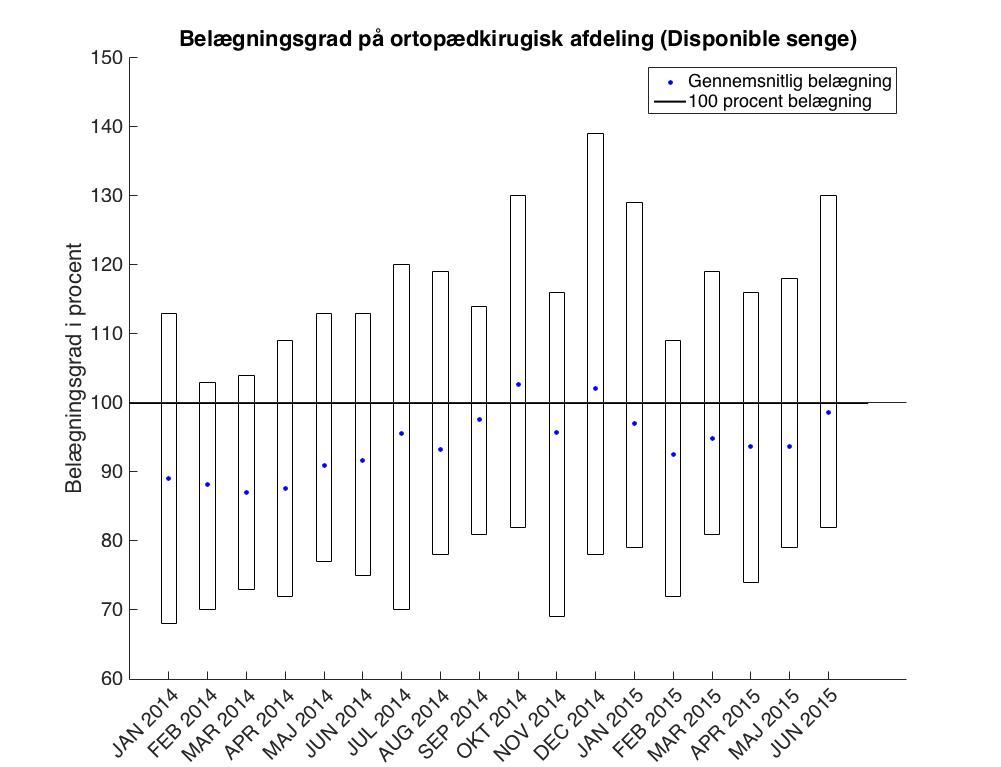
\includegraphics[scale=.45]{figures/maxminoverbelaeg.png}
	\label{maxminbelaeg}
	\flushleft
	\textit{Figuren viser minimums- og maksimumsbelægning på ortopædkirugisk, samt den gennemsnitlige belægning, fra januar $2014$ til juni $2015$ på ortopædkirugisk afdeling på Aalborg Universitetshospital.\cite{SDS2015}}
\end{figure}

\noindent
Som det ses på \figref{maxminbelaeg} er den gennemsnitlige belægning på ortopædkirugisk afdeling typisk under $100~\%$. Kun $2$ ud af de $18$ måneder har en gennemsnitlig belægning over $100~\%$. Det ses ligeledes at den maksimale belægning er over $100~\%$ i alle $18$ måneder. Dette tyder på at overbelægning på afdelingen forekommer i kortvarige episoder, frem for længerevarende perioder.\cite{SDS2015}

Dette underbygges af hyppigheden for overbelægning. Dette fremgår af \figref{antaldage}, som viser antallet af dage, hvor ortopædkirugisk afdeling på Aalborg Universitetshospital har haft en belægningsgrad over $100~\%$\cite{SDS2015}

\begin{figure}[H]
	\flushleft 
	\caption{Antal dage med belægningsgrad over $100$\% på ortopædkirugisk afdeling}
	\centering
	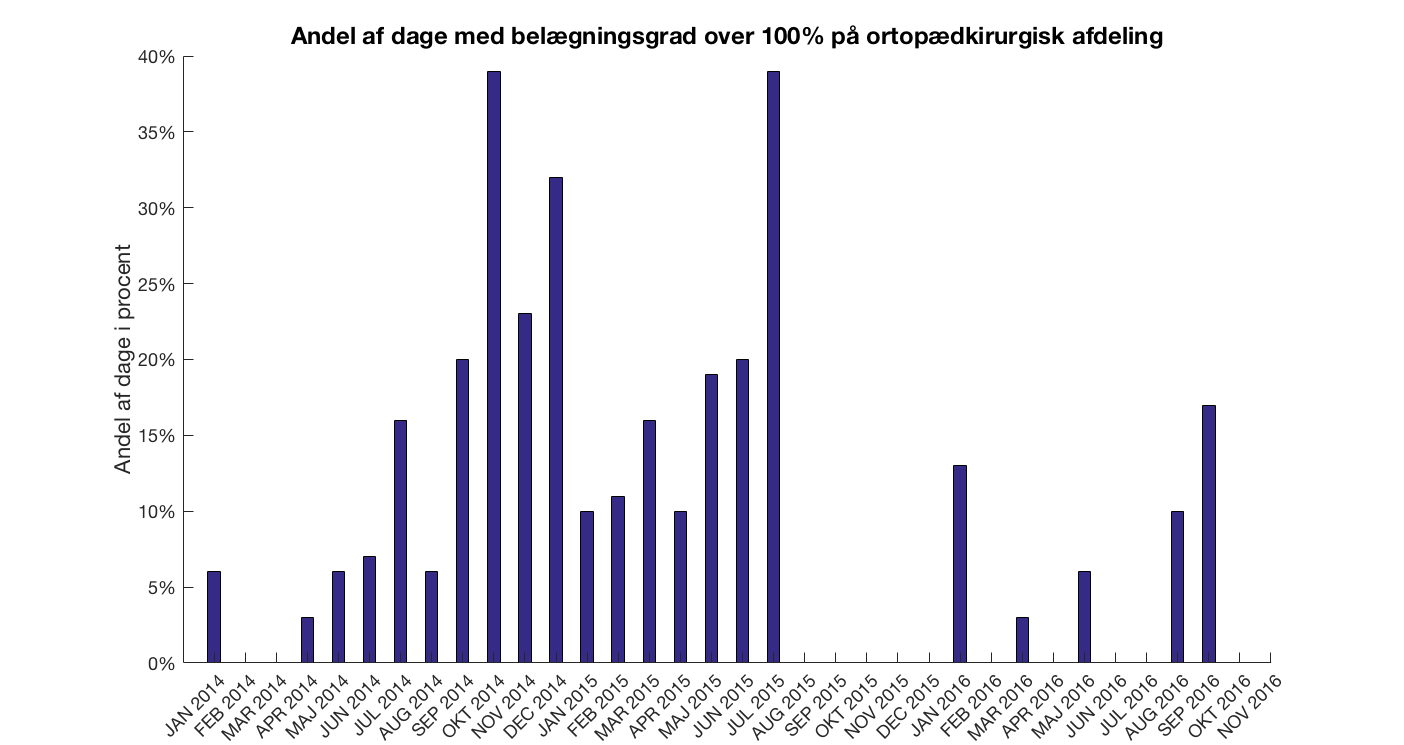
\includegraphics[scale=.7]{figures/antaldage.png}
	\label{antaldage}
	\flushleft
	\textit{Figuren antal dage med belægningsgrad over $100$\%, fra januar 2014 til juni 2015 på ortopædkirugisk afdeling på Aalborg Universitetshospital.\cite{SDS2015}}
\end{figure}